%!TEX root = Tesi.tex

\section{Bluetooth Low Energy}
\subsection{Introduzione}
Il Bluetooth Low Energy (BLE) è una tecnologia wireless introdotta nello standard 4.0, disegnata e commercializzata dal SIG\footnote{Bluetooth Special Interest Group: organizzazione che regolamenta e definisce gli standard  per la trasmissione dati tramite la tecnologia Bluetooth.}; ideata per trasmissioni di dati di breve dimensione, essa si differenzia dal Bluetooth classico per un inferiore consumo di energia, mantenendo la stessa portata trasmissiva.

\subsection{Banda Trasmissiva}
BLE opera alla stessa banda di frequenza del bluetooth classico,  2,400 - 2,4835 GHz, ma utilizza un numero inferiore di canali, 40 canali da 2 \si{\mega\hertz} l'uno.
Nel canale trasmissivo i dati sono trasmessi con una modulazione GFSK.\footnote{Gaussin Frequency Shift Keying, limita la larghezza dello spettro trasmissivo tramite un filtro di tipo Gaussiano.}
I bitrate trasmissivi sono limitati ai valori ${125\ \si{\kilo\bit/s}}$, ${1\ \si{\mega\bit/s}}$ o ${2\ \si{\mega\bit/s}}$.

\subsubsection{Mapping tra canali e frequenze}\label{channels}
Il protocollo BLE utilizza 40 canali fisici differenti per la trasmissione, con una numerazione che va da 0 a 39. Ogni canale ha una frequenza centrata in ${2402 + (k \cdot 2)\ \si{\mega\hertz}}$, dove k assume il valore del canale considerato.
Questi 40 canali si dividono in:
\begin{itemize}
\item 3 canali 0, 12 e 39 centrati nelle frequenze ${2402\ \si{\mega\hertz}}$, ${2426\ \si{\mega\hertz}}$ e ${2480\ \si{\mega\hertz}}$ ed utilizzati per l'Advertise.
\item i restanti 37 canali sono utilizzati per la trasmissione di dati che vengono utilizzati solo a connessione avvenuta per lo scambio di informazioni.
\end{itemize} 
La distribuzione di questi canali non è casuale: essi difatti sono i canali utilizzati da un dispositivo per far conoscere la propria presenza ai vicini, è quindi fondamentale che almeno uno di essi sia disponibile per la trasmissione, quindi privo di disturbi generati da altri sistemi che operano nella stessa banda trasmissiva. Sono stati distribuiti lontani tra di loro cercando di utilizzare tutta la banda disponibile per massimizzare la possibilità di avere un canale libero per la trasmissione. Un altro motivo della scelta è stato quello di poter facilitare la co-esistenza con la tecnologia Wifi, che utilizza la stessa banda per trasmettere, centrata principalmente nei canali Wifi 1, 6 e 11.


\begin{figure}[H]
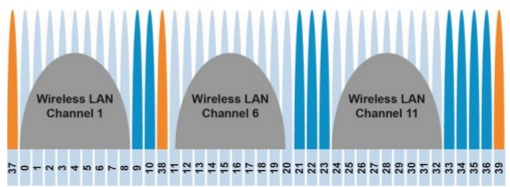
\includegraphics[width=370pt]{channel_mapping_wifi}
\centering
\caption{sovrapposizione alla banda BLE dei 3 canali usati principalmente nella comunicazione wifi; si noti come i 3 canali di advertise non rientrino in nessuno di questi 3 canali.}
\end{figure}




Per una miglior leggibilità ed un più facile utilizzo, si è scelto di mappare i canali reali con dei corrispondenti indici fittizi che vedono nelle numerazioni da 0 a 36 i canali data e 37, 38, 39 per i canali di Advertise;
\begin{itemize}
\item[-] canale fisico 0, di Advertise a frequenza 2402 MHz, mappato come canale 37.
\item[-] canale fisico 12, di Advertise a frequenza 2426 MHz, mappato come canale 38.
\item[-] canale fisico 39, di Advertise a frequenza 2480 MHz, mappato come canale 39. 
\item[-] canale fisico 1, di scambio dati a frequenza 2404 MHz, mappato come canale 0.
\item[-] \dots
\item[-] canale fisico 38, di scambio dati a frequenza 2478 MHz, mappato come canale 36.
\end{itemize}

\begin{figure}[H]
\caption{Distribuzione dei canali nella banda trasmissiva BLE, con il riferimento all'indice del canale mappato e la relativa frequenza centrale.}
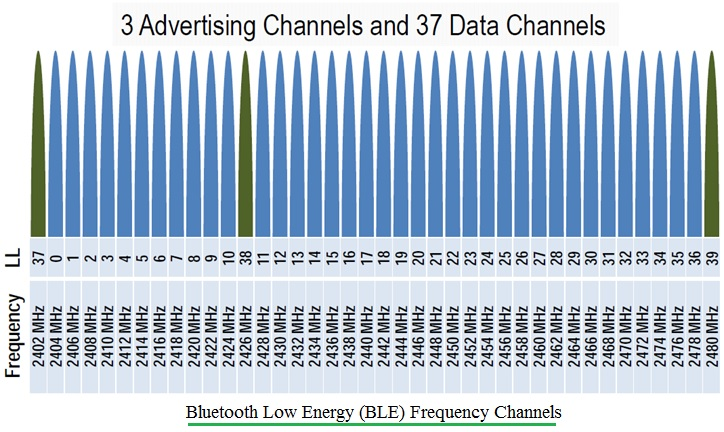
\includegraphics[width=350pt]{channel_mapping}
\centering
\label{channel_mapping}
\end{figure}




\subsubsection{Adaptive Frequency Hopping}\label{freqHopping}
Bluetooth Low Energy utilizza il \emph{Frequency Hopping}, una tecnica trasmissiva che consiste nel cambiare canale trasmissivo per ogni pacchetto inviato durante una trasmissione; l'utilizzo di questa tecnica permette di ridurre i problemi di interferenza con gli altri canali ed allo stesso tempo di aumentare la sicurezza delle trasmissioni. Esso è definito adattivo perché permette, in fase di connessione, di andare ad escludere determinati canali perché considerati troppo disturbati. L'algoritmo che regola questo cambio di canali è determinato da una formula che calcola il successivo canale in cui trasmettere, avendo come parametro l'ultimo canale usato e il numero di canali da saltare

\[Ch = (Ch_{-1} + HopIncrement)mod 37\]

Dove:
\begin{itemize}
\item[] \emph{Ch}: è il prossimo canale in cui trasmettere.
\item[] $Ch_{-1}$: è l'ultimo canale in cui si è trasmesso.
\item[] \emph{HopIncrement} : costante che indica il numero di canali da saltare, che viene scambiato dai dispositivi in fase di connessione.
\end{itemize}

\subsection{Stack protocollare}
Storicamente lo stack Bluetooth è diviso in 2 componenti fondamentali: il \emph{Controller} e l'\emph{Host}.
La parte di Controller è quella che si occupa di eseguire le componenti di basso livello dello stack necessarie per gestire i pacchetti scambiati a livello fisico e le loro temporizzazioni; la parte di Host comprende le componenti di alto livello tra cui profili e API\footnote{Application Program Interface: insieme di procedure utili a svolgere uno specifico compito}. La parte di Host, diversamente da quella di controllo, astrae dall'hardware ed è caratterizzata da una gestione meno rigida delle temporizzazioni.

L'\emph{HCI}\footnote{Host Controller Interface}, l'interfaccia tra Host e Controller si occupa di mettere in comunicazione queste due componenti fondamentali, utilizzando canali comunicativi quali UART o USB.
Se i due componenti sono montati su uno stesso chip, come nel caso dei SoC\footnote{System on a Chip: sistema completamente contenuto su un solo Chip}, allora l'interfaccia HCI è opzionale e può essere omessa.

\begin{figure}[H]
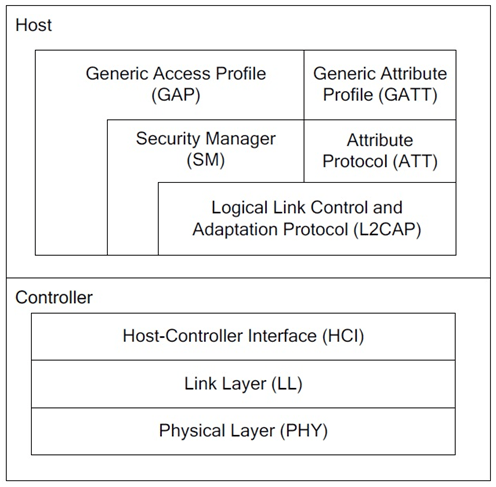
\includegraphics[scale=0.6]{stack_ble.png}
\centering
\end{figure}

\begin{itemize}
\item Physical Layer (PHY): è il livello fisico, ovvero l'etere; lavora nella banda di frequenza 2,4 GHz ISM\footnote{Industrial, Scientific and Medical: frequenze riservate alle applicazioni di radiocomunicazioni non commerciali, ovvero per uso industriale, scientifico e medico.} Si compone di 40 canali da 2 MHz ognuno suddivisi in 3 per advertising e 37 per lo scambio dati.

\item Link Layer (LL): si occupa della gestione della sequenza e della temporizzazione dei pacchetti scambiati. Dialoga con i nodi vicini e scambia informazioni quali i parametri di connessione e controllo di flusso.\linebreak 
\'E una macchina a stati che si compone di 5 stati: Standby, Advertising, Scanning, Initiating, Connection. 

\begin{figure}[H]
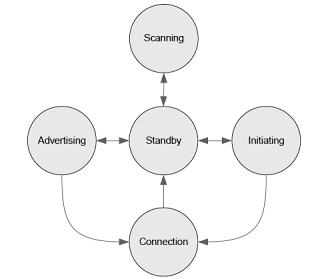
\includegraphics[scale=0.7]{LL_states}
\centering
\end{figure}

\begin{itemize}

\item Advertising: il dispositivo rende noto agli ascoltatori della propria presenza, indicando la disponibilità ad una connessione ed inviando alcune informazioni utili.

\item Scanning: il dispositivo è in ascolto di tutte le informazioni trasmesse sui canali di advertise.

\item Initiating: un dispositivo in ascolto individua un Advertise di suo interesse ed indica la sua volontà di connettersi.

\item Connection: due o più dispositivi sono connessi.

\item Standby: il dispositivo è in uno stato di attesa caratterizzato da un basso consumo energetico.

\end{itemize}

Lo stato di Scanning può essere attivo (richiede informazioni aggiuntive) o passivo; Lo stato Connection anch'esso si divide in 2 sottostati: Central e Peripheral.

\item Logical Link Control and Adaptation Protocol (L2CAP): fornisce servizi sui dati ai livelli superiori, come ad esempio il Security Manager Protocol o l'Attribute Protocol. \'E responsabile inoltre della segmentazione e ricostruzione dei pacchetti da e verso i livelli inferiori.

\item Security Manager (SM): è responsabile del pairing dei dispositivi e della distribuzione delle chiavi crittografiche; BLE utilizza lo standard AES-128 bit per la cifratura dei dati ed il sistema di pairing per la distribuzione delle chiavi.

\item Attribute Protocol (ATT): gestisce la distribuzione delle informazioni riguardanti le coppie attributo-valore presenti in un device peripheral (Server)

\item Generic Access Profile (GAP): controlla \emph{advertising} e \emph{connection} . Divide i dispositivi bluetooth low energy in:
\begin{itemize}
\item Peripheral: normalmente dispositivi dotati di una limitata capacità di calcolo, come ad esempio un sensore di temperatura.
\item Central: dispositivo che gestisce la rete bluetooth e che richiede una maggiore capacità di calcolo; mentre un dispositivo periferico può avere una connessione con un solo dispositivo centrale, un centrale può gestire più dispositivi periferici andando a creare una Piconet\footnote{Rete Bluetooth composta da massimo otto dispositivi in relazione master-slave e fino a 255 dispositivi in modalità inattiva o parcheggio.}
\end{itemize} 

\item Generic Attribute Profile (GATT): entra in gioco a connessione avvenuta, definisce il modo in cui 2 dispositivi BLE scambiano dati utilizzando i concetti di \emph{Services} e \emph{Characteristics}.

\begin{itemize}
\item GATT server: è un peripheral device, che tramite il protocollo ATT permette al central di conoscere i dati che ha memorizzato in strutture di tipo service-characteristic.
\item GATT client: è il central device, che gestisce le comunicazioni e che richiede ai server periferici i dati raccolti.
\end{itemize}
\end{itemize}

\subsection{Formato dei pacchetti}

Il Link Layer (LL) ha un unico formato per tutti i pacchetti scambiati, che quindi è uguale sia per i pacchetti di tipo Advertise, sia per i pacchetti di scambio di dati.
In figura \ref{pacchetto_LL} è mostrato il formato dei pacchetti

\begin{figure}[H]
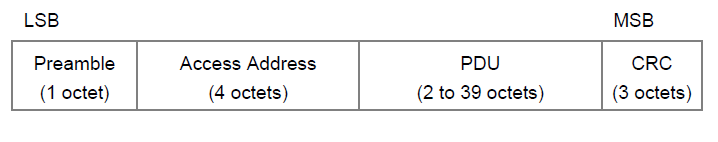
\includegraphics[width=350pt]{pacchetto_LL}
\centering
\caption{formato dei pacchetti Link Layer}
\label{pacchetto_LL}
\end{figure}

\begin{itemize}

\item \textbf{Preamble}: composto da 8 bit, è utile al ricevitore del pacchetto per sincronizzarsi sulla frequenza portante, e per impostare l'\emph{Automatic Gain Control} (AGC).
I pacchetti di Advertise hanno come preambolo $10101010b$. Per i pacchetti data il valore del preambolo è determinato dal LSB\footnote{Less Significant Bit, il bit meno significativo.} dell'Access Address; se è 1 il preambolo è $01010101b$, se è 0 il preambolo vale $10101010b$


\item \textbf{Access Address}: \label{access_address}
Campo composto da 4 Byte; per i pacchetti di Advertise assume un valore costante pari a 0x8E89BED6. Per le trasmissioni di dati l'Access Address deve essere diverso per ogni connessione; dovrebbe essere un valore casuale (con alcune restrizioni) di 32 bit generato dal dispositivo che inizia la connessione ed inviato al secondo dispositivo durante la connessione tramite il pacchetto di Connection Request. 

\item \textbf{PDU}:
Composta da un numero variabile da 2 a 39 byte, è l'acronimo di Protocol Data Unit, ovvero l'unità di informazione scambiata. A seconda che si abbia un pacchetto di Advertise o un pacchetto dati, la PDU assume una struttura differente. I vari tipi di PDU sono trattati nel capitolo \ref{pdus}

\item \textbf{CRC}:
Alla fine di ogni pacchetto Link Layer c'è un CRC,Il cyclic redundancy check (ovvero controllo a ridondanza ciclica), di 24 bit. Esso serve per rilevare eventuali errori di trasmissione, quindi per sapere se il pacchetto ricevuto è corrotto.
Il CRC viene calcolato sul campo PDU, partendo dal LSB; il polinomio per il calcolo è:
\[x^24 + x^10 + x^9 + x^6 + x^4 + x^3 + x + 1\] 
Se il calcolo del CRC viene fatto su un PDU di tipo Advertise, deve essere inizializzato con il valore 0x555555;
Se viene fatto su un pacchetto dati, deve essere inizializzato ad un valore scambiato in fase di comunicazione (di 3 Byte), contenuto nella Connection Request.
In posizione 0 va inserito il bit meno significativo del valore di inizializzazione, ma il CRC viene inviato con il bit più significativo (bit 23) in posizione iniziale.

\end{itemize}



\subsection{PDU dei canali di Advertise}\label{pdus}
Il PDU di un pacchetto di Advertise si compone di un header di 16 bit ed un payload con una lunghezza variabile dai 6 ai 37 Byte.

\begin{figure}[H]
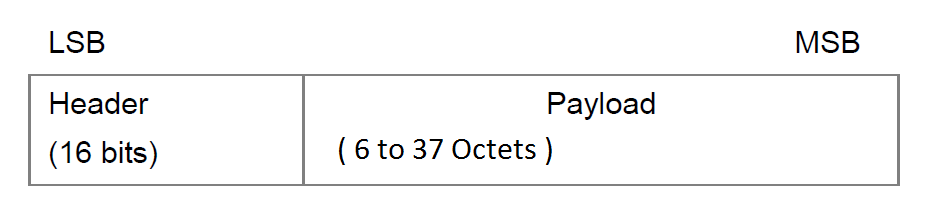
\includegraphics[width=315pt]{Advertising_pdu}
\centering
\caption{Advertising PDU}
\end{figure}

\noindent L'Header di questo PDU si compone di vari campi, come mostrato in figura \ref{Advertising_pdu_header}

\begin{figure}[H]
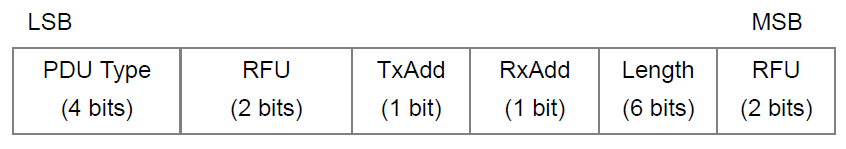
\includegraphics[width=350pt]{Advertising_pdu_header}
\centering
\caption{Advertising PDU Header}
\label{Advertising_pdu_header}
\end{figure}

Il campo PDU type verrà approfondito in seguito, assieme al significato dei campi TxAdd e RxAdd; Il campo length, di 6 bit quindi con un valore massimo di 63, ma settabile dalle specifiche ad un valore massimo di 37, indica i Byte di dimensione del Payload.


\subsubsection{PDU type}

\begin{figure}[H]
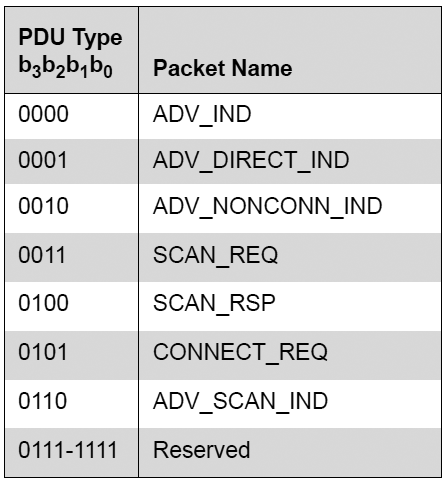
\includegraphics[width=220pt]{advertising_pdu_type}
\centering
\caption{Codifiche dei possibili tipi di PDU di un pacchetto di Advertise}
\end{figure}
 
I vari tipi di PDU di un canale di Advertise si raggruppano in 3 insiemi distinti: Advertising PDU, Scanning PDU e Initiating PDU.

\subsubsection{Advertising PDU}

Questi PDU sono inviati da un dispositivo in stato di Advertise e ricevuti da un sistema in stato di scanning.

\begin{itemize}
\item ADV\_ IND: evento di advertising che notifica la disponibilità ad una connessione indiretta, ovvero senza specifiche sull'indirizzo da cui ricevere la richiesta di connessione.
Il payload di questo tipo di PDU è mostrato in figura \ref{adv_ind_payload}, il campo TxAdd dell'header se settato a 1 indica che l'indirizzo del campo AdvA del payload è casuale, se settato a 0 esso è pubblico.

\begin{figure}[H]
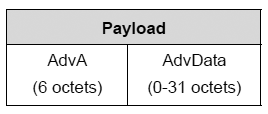
\includegraphics[width=185pt]{adv_ind_payload}
\centering
\caption{Payload di un PDU di tipo ADV\_ IND }
\label{adv_ind_payload}
\end{figure}

Si compone dei campi AdvA di 6 byte, che indica l'indirizzo, pubblico o privato, dell'advertiser, ovvero di chi sta inviando il pacchetto, e il campo AdvData che contiene eventuali informazioni aggiuntive ed ha una lunghezza massima di 31 Byte.

\item ADV\_ DIRECT\_ IND: evento di connessione diretta, in cui nel payload, mostrato in figura \ref{adv_direct_ind_payload} è indicato l'indirizzo da cui ci si aspetta una connessione. Il campo TxAdd dell'header se settato a 1 indica che l'indirizzo del campo AdvA del payload è casuale, se settato a 0 esso è pubblico;
il campo RxAdd dell'header se settato a 1 indica che l'indirizzo del campo InitA del payload è casuale, se settato a 0 esso è pubblico. 

\begin{figure}[H]
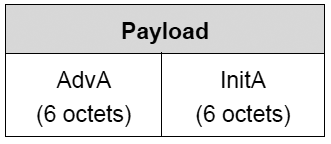
\includegraphics[width=170pt]{adv_direct_ind_payload}
\centering
\caption{Payload di un PDU di tipo ADV\_ DIRECT\_ IND }
\label{adv_direct_ind_payload}
\end{figure}

Il campo AdvA contiene l'indirizzo dell'Advertiser, sia esso pubblico o privato, ed il campo InitA indica l'indirizzo da cui ci si aspetta la connessione. Il payload di questo tipo non contiene nessuna informazione aggiuntiva.

\item ADV\_ NONCONN\_ IND: evento di non connessione; utilizzato per applicazioni di tipo BEACON, ovvero per condividere informazioni a chiunque è in ascolto. Nel  payload, mostrato in figura \ref{adv_nonconn_ind_payload} è indicato l'indirizzo dell'Advertiser. Il campo TxAdd dell'header se settato a 1 indica che l'indirizzo del campo AdvA del payload è casuale, se settato a 0 esso è pubblico;

\begin{figure}[H]
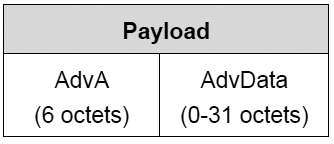
\includegraphics[width=170pt]{adv_nonconn_ind_payload}
\centering
\caption{Payload di un PDU di tipo ADV\_ NONCONN\_ IND }
\label{adv_nonconn_ind_payload}
\end{figure}

Il campo AdvA contiene l'indirizzo dell'Advertiser, sia esso pubblico o privato, ed il campo AdvData che contiene le informazioni da condividere ed ha una lunghezza massima di 31 Byte.

\item ADV\_ SCAN\_ IND: evento di connessione indiretta in cui si informa che si hanno ulteriori informazioni da condividere; chi è interessato a queste informazioni manderà all'Advertiser un PDU di tipo SCAN\_ REQ, e l'advertiser risponderà con un PDU di tipo SCSN\_ RSP contenente le informazioni aggiuntive. Nel  payload, mostrato in figura \ref{adv_scan_ind_payload} è indicato l'indirizzo dell'Advertiser. Il campo TxAdd dell'header se settato a 1 indica che l'indirizzo del campo AdvA del payload è casuale, se settato a 0 esso è pubblico;

\begin{figure}[H]
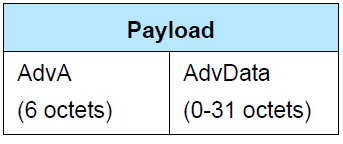
\includegraphics[width=170pt]{adv_scan_ind_payload}
\centering
\caption{Payload di un PDU di tipo ADV\_ SCAN\_ IND }
\label{adv_scan_ind_payload}
\end{figure}

Il campo AdvA contiene l'indirizzo dell'Advertiser, sia esso pubblico o privato, ed il campo AdvData che contiene le eventuali informazioni da condividere ed ha una lunghezza massima di 31 Byte.

\end{itemize}

\subsubsection{Scanning PDU}

\begin{itemize}

\item SCAN\_ REQ: dopo aver ricevuto un pacchetto di Advertise, uno scanner in stato attivo può richiedere eventuali informazioni aggiuntive con questo tipo di PDU. Il campo TxAdd dell'header se settato a 1 indica che l'indirizzo del campo AdvA del payload, figura \ref{scan_req_payload} è casuale, se settato a 0 esso è pubblico; il campo RxAdd dell'header se settato a 1 indica che l'indirizzo del campo InitA del payload è casuale, se settato a 0 esso è pubblico.

\begin{figure}[H]
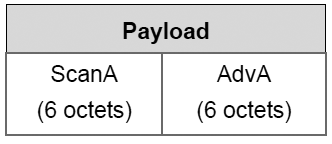
\includegraphics[width=170pt]{scan_req_payload}
\centering
\caption{Payload di un PDU di tipo SCAN\_ REQ }
\label{scan_req_payload}
\end{figure}

Nel campo ScanA viene indicato l'indirizzo del device che genera questo pacchetto di SCAN\_ REQ, mentre nel campo AdvA viene indicato l'indirizzo del dispositivo in stato di Advertise a cui è destinato questo pacchetto.

\item SCAN\_ RSP: dopo aver ricevuto un pacchetto di tipo SCAN\_ REQ destinato a lui, l'Advertiser può decidere di adempire alla richiesta inviando questo tipo di PDU con le informazioni aggiuntive che vuole fornire. Il campo TxAdd dell'header se settato a 1 indica che l'indirizzo del campo AdvA del payload, figura \ref{scan_rsp_payload} è casuale, se settato a 0 esso è pubblico;

\begin{figure}[H]
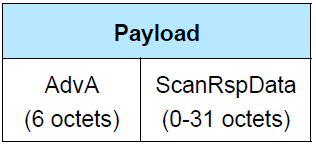
\includegraphics[width=155pt]{scan_rsp_payload}
\centering
\caption{Payload di un PDU di tipo SCAN\_ RSP }
\label{scan_rsp_payload}
\end{figure}

Nel campo AdvA viene indicato l'indirizzo del device che genera questo pacchetto di SCAN\_ RSP, mentre nel campo ScanRspData viene inserita l'eventuale informazione aggiuntiva da condividere, con lunghezza massima di 31 Byte.

\end{itemize}

\subsubsection{Initiating PDU}\label{conn_req}

CONNECT\_ REQ: inviata da un dispositivo in stato di scanning, consente a quest'ultimo di effettuare una connessione con il dispositivo in stato di Advertising che ha dichiarato la sua disponibilità a connettersi.

\begin{figure}[H]
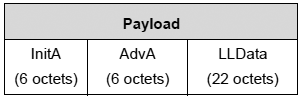
\includegraphics[width=230pt]{conn_req_payload}
\centering
\caption{Payload di un PDU di tipo CONNECT\_ REQ }
\label{conn_req_payload}
\end{figure}

Il payload è mostrato in figura \ref{conn_req_payload} e si compone di 3 campi principali: 
\begin{itemize}
\item InitA (6 Byte): l'indirizzo del dispositivo che ha avviato la connessione, ovvero chi ha mandato il pacchetto di CONN\_ REQ;
\item AdvA (6 Byte): l'indirizzo dell'Advertiser, quello a cui vuole connettersi chi ha iniziato la connessione;
\item LLData (22 Byte): è il cuore del pacchetto; qui si trovano tutte le informazioni sui parametri da usare durante la connessione.
\end{itemize}

Una trattazione riservata va fatta al campo LLData, mostrato il figura \ref{lldata} che si compone di 10 campi.

\begin{figure}[H]
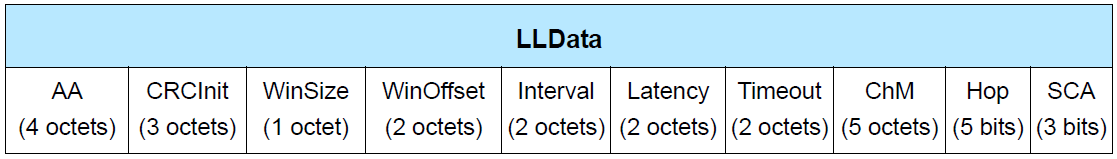
\includegraphics[width=400pt]{lldata}
\centering
\caption{Campi di una struttura LLData di un pacchetto PDU di tipo CONNECT\_ REQ}
\label{lldata}
\end{figure}


Nel dettaglio i campi sono:
\begin{itemize}
\item AA (4 Byte): il campo contiene l'Access Address (specificato nel capitolo \ref{access_address}) utilizzato per tutta la durata della connessione.
\item CRCInit (3 Byte): contiene il valore a cui inizializzare il calcolo del CRC per la connessione a livello Link Layer. \'E un valore casuale, generato dal dispositivo che avvia la connessione.
\item WinSize: determina il valore di ${transmitWindowSize = WinSize \cdot 1.25\ \si{ms}}$, spiegato in dettaglio nel paragrafo \ref{connState}.
\item WinOffset: determina il valore di ${transmitWindow\mathit{Offs}et =
Win\mathit{Offs}et \cdot 1.25\ \si{ms}}$, spiegato in dettaglio nel paragrafo \ref{connState}.
\item Interval: determina il valore di ${connInterval = Interval \cdot 1.25\ \si{ms}}$, spiegato in dettaglio nel paragrafo \ref{connState}.
\item Latency: indica il numero di volte che lo slave può non rispondere nella finestra di \emph{connInterval} pur mantenendo valida la connessione (\emph{connSlaveLatency}).
\item Timeout: determina il valore di ${connSupervisionTimeout = Timeout \cdot 10\ \si{ms}}$, spiegato in dettaglio nel paragrafo \ref{timeout}.
\item ChM (5 byte): indica quali tra i canali destinati allo scambio di informazioni durante una connessione (vedi capitolo \ref{channels}) devono essere usati. Ogni canale è rappresentato da un bit, il cui valore 1 indica che verrà utilizzato, mentre il valore 0 che non lo sarà. I bit 37, 38 e 39, che indicano i canali di Advertise, non sono utilizzati (RFU).
\item Hop(5 bit): il campo hop indica il valore di HopIncrement (Capitolo \ref{freqHopping}) che verrà utilizzato dall'algoritmo per  determinare di volta in volta il canale su cui trasmettere.
\item SCA(3 bit): determina l'accuratezza dello \emph{Sleep Clock}.

\end{itemize}

\subsection{PDU dei canali Data}
Il PDU che viene inviato nei canali di scambio dati, ovvero dal canale 0 al canale 36, ha la struttura mostrata in figura \ref{data_pdu} e si compone di un header da 16 bit, payload e un campo MIC (\emph{Message Integrity Check}) opzionale.

\begin{figure}[H]
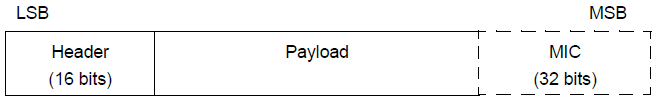
\includegraphics[width=350pt]{data_pdu}
\centering
\caption{PDU di un pacchetto Data}
\label{data_pdu}
\end{figure}

L'header di questo pacchetto ha 5 campi, mostrati in figura \ref{data_pdu_header}, analizzati nel dettaglio di seguito:

\begin{figure}[H]
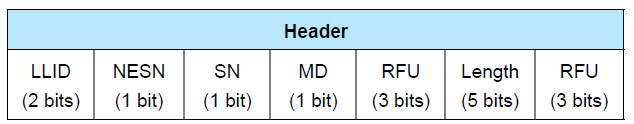
\includegraphics[width=370pt]{data_pdu_header}
\centering
\caption{Header di un PDU di tipo Data}
\label{data_pdu_header}
\end{figure}

\begin{samepage}

\begin{itemize}

\item LLID: da informazioni sul tipo di pacchetto, che può essere di \emph{LL Data} o \emph{LL Control}

\begin{itemize}
\item 00b: non utilizzato.
\item 01b: PDU di tipo LL Data, può essere la continuazione di un messaggio L2CAP oppure un PDU vuoto, con campo length posto a 0, usato per il controllo.
\item 10b: PDU di tipo LL Data, può essere un messaggio L2CAP completo o il suo inizio.
\item 11b: PDU di tipo LL Control.
\end{itemize}

\item NESN (1 bit): Next Expected Sequence Number, usato come acknowledge, ovvero per indicare che l'ultimo pacchetto ricevuto è stato ricevuto correttamente.
\item SN (1 bit): Sequence Number, usato per conoscere se il pacchetto che si sta inviando è un nuovo pacchetto o la ritrasmissione di uno precedente.
\item MD (1 bit): More Data, indica se il pacchetto è la continuazione di uno precedente o  contiene nuove informazioni.
\item Length (5 bit): come per l'header di un pacchetto di Advertise, indica la lunghezza del payload ed eventualmente quella del campo MIC se presente; il payload ha una lunghezza massima di 27 Byte, il MIC è fisso a 4 Byte, quindi il campo length varia da 0 a 31 Byte.

\end{itemize}
\end{samepage}

\subsection{Stato di connessione}\label{connState}
Il Link Layer entra in uno stato di connessione quando l'initiator invia un pacchetto di tipo CONNECT\_ REQ (Capitolo \ref{conn_req}); dopo aver ricevuto il pacchetto la connessione viene considerata creata ma non stabilita. Dopo che viene inviato il primo pacchetto dati la connessione si considera stabilita.
Durante una connessione i due dispositivi assumono due ruoli ben distinti:
\begin{itemize}
\item Chi ha inviato il pacchetto di CONNECT\_ REQ assumerà il ruolo di \emph{Master} in posizione di dispositivo Centrale
\item L'altro partecipante alla connessione sarà lo \emph{Slave} ed assumerà la posizione di dispositivo periferico.
\end{itemize}
Una connessione si compone di più eventi di connessione; Master e Slave possono scambiarsi dati sono all'interno di un evento, il quale deve contenere almeno un pacchetto inviato dal Master. Lo slave deve sempre rispondere quando riceve un pacchetto dal Master, anche nel caso in cui il pacchetto abbia un CRC non valido; se il master non riceve un pacchetto in risposta dallo slave, deve chiudere la connessione. Ulteriormente la connessione può essere chiusa volontariamente sia dallo Slave che dal Master.


La temporizzazione di una connessione è scandita da due parametri fondamentali: connection event interval (\emph{connInterval}) e slave latency (\emph{connSlaveLatency}. L'instante dell'inizio di un evento di connessione è chiamato anchor point; in questo istante il master deve cominciare a trasmettere un pacchetto.
Il connInterval deve essere un multiplo di 1,25 ms con un valore da 7,5 ms a 4 secondi.
Il connSlaveLatency indica il numero di eventi di connessione che lo slave può ignorare pur mantenendo attiva la connessione; è un valore intero che va da 0 a 500 ed è calcolato come $((connSupervisionTimeout/connInterval) - 1)$
\linebreak
Sia Master che Slave devono avere un contatore a 16 bit (\emph{connEventCounter}), settato a 0 al primo pacchetto inviato durante il primo evento di connessione, inviato dal master; viene incrementato ciclicamente ad ogni evento di connessione.

\subsubsection{Supervision Timeout}\label{timeout}
Una connessione può terminare anche per fattori fisici riguardanti i dispositivi, come ad esempio una distanza troppo elevata, interferenze od una mancanza di potenza. Per determinare tali eventi, sia Master che Slave devono utilizzare un timer chiamato TLLConnSupervision. 
Se in fase di connessione questo timer raggiunge il valore di $6 \cdot connInterval$ prima che la connessione sia stabilita, essa si considera fallita.
A connessione stabilita, il parametro connection supervisor timeout (\emph{connSupervisionTimeout}) definisce il tempo massimo che deve passare tra la ricezione di due PDU di tipo data successive; Deve essere un multiplo di 10 ms con un valore compreso tra 10 ms e 32 s calcolato come $(1 + connSlaveLatency) \cdot connInterval$.
Se durante una connessione, il timer raggiunge il valore di connSupervisionTimeout, la connessione deve considerarsi persa.

\subsubsection{Transmit Window}
In figura \ref{transmit_window} è mostrato un evento di connessione a livello Link Layer, in cui sono visualizzati sia i pacchetti di Advertise con la relativa CONNECT\_ REQ, sia i primi pacchetti di dati scambiati. Il dispositivo Master può settare l'Anchor Point a suo piacimento, per gestire eventuali altre connessioni a cui partecipa; l'Anchor Point viene settato quando il Master invia il primo pacchetto dati nella transmitWindow. Essa inizia a 1,25 ms + \emph{transmitWindowOffset} dopo aver ricevuto il PDU della CONNECT\_ REQ; il primo pacchetto non deve essere inviato più tardi di 1.25 ms + transmitWindowOffset + transmitWindowSize.

\begin{figure}[H]
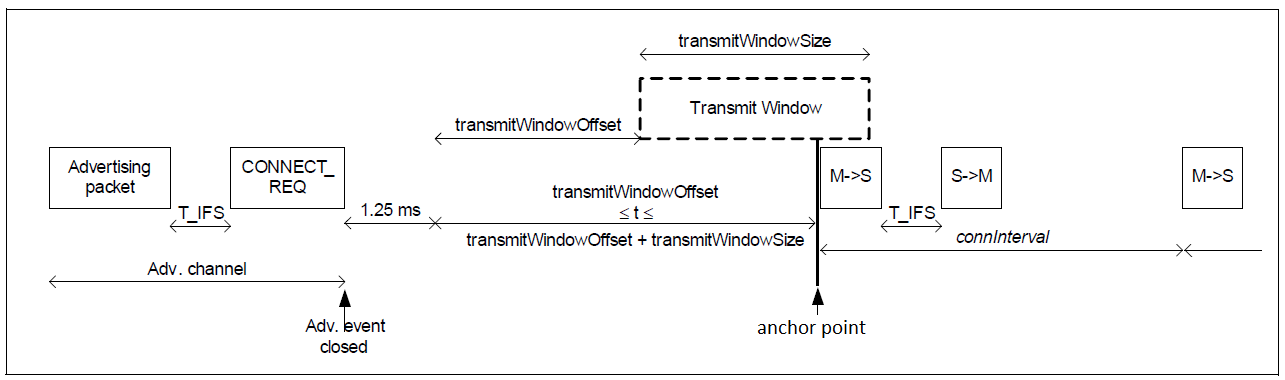
\includegraphics[width=400pt]{transmit_window}
\centering
\caption{Schema di temporizzazione di un evento di connessione. }
\label{transmit_window}
\end{figure}

Il parametro \emph{transmitWindowSize} è un multiplo di 1,25 ms e varia da 1,25 ms a meno di 10 ms e meno di (connInterval - 1.25 ms). Il \emph{transmitWindowOffset} è sempre un multiplo di 1,25 e va da 0 a connInterval.
L'intervallo di tempo tra due pacchetti consecutivi sullo stesso canale, come ad esempio la richiesta del Master e la risposta dello Slave, è chiamato Inter Frame Space; è definito come il tempo trascorso dalla fine dell'invio dell'ultimo bit del primo pacchetto all'inizio dell'invio del primo bit del secondo pacchetto. Abbreviato con l'etichetta T\_ IFS ha un valore di 150 $\mu s$

\subsection{Bit Ordering}\label{endian_bit}
L'ordine dei bit nei campi dei vari pacchetti seguono le specifiche del formato Little Endian, ovvero vengono scritti prima i Byte meno significativi ed in ordine fino ai più significativi. Si applicano inoltre le seguenti regole:

\begin{itemize}
\item Il bit meno significativo viene indicato con b0
\item Il bit meno significativo è il primo a essere inviato nell'etere
\item Nelle varie illustrazioni, l'LSB è mostrato sulla sinistra
\end{itemize}

Eventuali valori binari in ordine classico, quindi con il bit più significativo a sinistra, saranno indicati con l'appendice \lq b\rq, come ad esempio $01010101b$ che è un possibile valore per il preambolo.

Campi composti da più di un Byte, ad eccezione dei campi CRC e MIC, devono essere trasmessi con il Byte meno significativo prima ed ogni Byte con il proprio bit meno significativo iniziale.
Per il campo CRC e MIC sono scritti con il byte più significativo a sinistra.

\subsection{Device Address}
I dispositivi sono unicamente identificati dal Device Address; è un indirizzo composto da 6 Byte e può essere pubblico o casuale.
L'indirizzo di tipo pubblico, deve essere creato in accordo con lo standard IEEE 802-2001; un indirizzo di questo tipo è così composto:
\begin{itemize}
\item company assigned: campo assegnato dal costruttore dell'hardware, compone i 24 bit meno significativi dell'indirizzo.
\item company id: identifica univocamente il costruttore dell'hardware, compone i 24 bit più significativi dell'indirizzo.
\end{itemize}
L'indirizzo di tipo casuale si divide nei 2 campi:
\begin{itemize}
\item Hash: occupa i 24 bit meno significativi, è ottenuto come funziona Hash a partire dai 3 Byte più significativi.
\item Random: generato casualmente, compone i 24 bit più significativi dell'indirizzo.
\end{itemize}



